\documentclass[a4paper,11pt]{article}
\usepackage{graphicx}
\usepackage{float}
\usepackage{subfig}
\usepackage{geometry}
\usepackage{amsmath,amssymb}
\usepackage{amsthm}
\usepackage{bbold}
\usepackage{mathtools}
\usepackage{braket}
\usepackage{booktabs}
\usepackage[table,xcdraw]{xcolor}
\usepackage[utf8]{inputenc}
\usepackage{cite}
\usepackage[english]{babel}
\usepackage{lipsum}
\usepackage{setspace}
%\usepackage{minted}
\usepackage{xcolor}
\newcommand{\R}{\mathbb{R}}
\usepackage{hyperref}
\hypersetup{colorlinks=true,linkcolor=blue}
\geometry{a4paper, top=2.5cm, bottom=2.5cm, left=3cm, right=2.5cm}

\begin{document}
\author{Catalano Giuseppe, Cerrato Nunzia}
\title{Numerical Linear Algebra Homework Project 2:\\Least Squares, Orthogonalization, and the SVD}
\date{}
\maketitle

\section*{Problem 1}
\textbf{(1)} Suppose we are given $m$ pairs of data points, $(x_1,y_1),\dots,(x_m,y_m)$. We want to find a linear combination of prescribed functions $\phi_1, \dots, \phi_n$ whose values at the points $x_i \in [a,b] $, $1\le i \le m$, approximate the values $y_1,\dots, y_m$ as well as possible. More precisely, the problem is to find a function of the form $f(x) = \alpha_1 \phi_1(x) + \dots + \alpha_n \phi_n(x) $ such that 
\begin{equation}
	\sum_{i=1}^{m} \left[ y_i - f(x_i) \right]^2 \le \sum_{i=1}^{m} \left[ y_i - g(x_i) \right]^2\ \ \ \forall g \in \text{Span}(\phi_1,\dots,\phi_n),
\end{equation}
where, usually, $m>n$. It is possible to rephrase the problem as:
\begin{equation}\label{eq: initial definition of the minimization problem}
	f = \arg \min_{f\in \text{Span}(\phi_1,\dots,\phi_n)} \sum_{i=1}^{m} \left[ y_i - f(x_i) \right]^2.
\end{equation}
Now we can define a column vector $\textbf{z} \in \R^n$ such that:
\begin{equation}\label{key}
	[\textbf{z}]_i = \alpha_i
\end{equation}
and a matrix $A$ such that:
\begin{equation}\label{key}
	[A\textbf{z}]_i = f(x_i) = \alpha_1 \phi_1(x_i) + \dots + \alpha_n \phi_n(x_i).
\end{equation}
In this way, the element of the $i-th$ row and $j-th$ column of the matrix $A$ is:
\begin{equation}\label{key}
	[A]_{ij} = a_{ij} = \phi_j(x_i).
\end{equation}
Finally, defining a column vector $\textbf{b} \in \R^n$ such that:
\begin{equation}\label{key}
	[\textbf{b}]_i = y_i
\end{equation}
we can rewrite the \eqref{eq: initial definition of the minimization problem} as follows:
\begin{equation}\label{key}
	\tilde{\textbf{z}} = \arg \min_{\textbf{z}\in \R^n} \lVert \textbf{b} - A \textbf{z} \rVert_2^2 =  \arg \min_{\textbf{z}\in \R^n} \lVert \textbf{b} - A \textbf{z} \rVert_2,
\end{equation}
where the function $f$ can be built from $\tilde{\textbf{z}}$.

\noindent \textbf{(2)} Now we suppose to take $\phi_k = x^{k-1}$, $1 \le k \le n$. Under this assumption, the matrix $A$ takes the form:
\begin{equation}\label{key}
	A = \begin{bmatrix}
		x_1^0 & \cdots & x_1^{n-1}  \\
		\vdots & \ddots & \vdots \\
		x_m^0 & \cdots  & x_m^{n-1}
	\end{bmatrix}.
\end{equation}
We want to prove that, assuming that $x_i\neq x_j$ for $i \neq j$, $A$ has full rank: $\text{rank}(A) = n$.\\
Proof: Proving that $\text{rank}(A) = n$ is equivalent to prove that $\dim(\ker(A)) = 0$, that means that $\nexists \textbf{v} \in \R^n \text{ s.t. } \textbf{v} \in \ker(A)$. We want to prove this statement by contraddiction, therefore, we look for a vector $\textbf{v} \in \R^n$, with $\textbf{v} \neq \underline{0}$, such that $A\textbf{v}=\underline{0}$, that means:
\begin{equation}\label{key}
	\left\lbrace 
	\begin{split}
		&  v_1 x_1^0 + \dots + v_n x_1^{n-1} = 0\\
		& \vdots  \\
		&  v_1 x_m^0 + \dots + v_n x_m^{n-1} = 0 
	\end{split} \right.  .
\end{equation}
Defining the polynomial 
\begin{equation}\label{key}
	p^{(n-1)}_{\textbf{v}}(x) = \sum_{i=1}^{n} v_i x^{i-1}
\end{equation}
we can observe that, for any choice of $\textbf{v} \neq \underline{0}$, $p^{(n-1)}_{\textbf{v}}(x)$ admits at most $n-1$ different roots, therefore $\nexists \textbf{v} \neq \underline{0}$ such that $A\textbf{v}=\underline{0}$. This concludes the proof. \qedsymbol

\noindent \textbf{(3)} Consider the problem of finding the best fit with a quadratic function $f(x) = \alpha_1 + \alpha_2 x + \alpha_3 x^2$ for the following data:\\
\begin{center}	
\begin{tabular}{c|c|c|c|c|c|c|c|c|c}
	$x_i$& 8 & 10 & 12 & 16 & 20 & 30 & 40 & 60 & 100 \\
	\hline
	$y_i$& 0.88 & 1.22 & 1.64 & 2.72 & 3.96 & 7.66 & 11.96 & 21.56 & 43.16 \\
\end{tabular}.
\end{center}
In the following we report the code that solves the normal equations:
\begin{equation}\label{key}
	A^T A \textbf{v} = A^T \textbf{b}
\end{equation}
using the Cholesky factorization algorithm and then compares the result with the one found using the QR factorization of the matrix $A$.

\noindent *** INSERIRE CODICE ***

\noindent Using the previous functions we have computed the solution to the minimization problem, obtaining the following results:\\
\begin{tabular}{cc}
	Cholesky:  &$x = [-1.91914925269909,\   0.278213536291725,\ 0.001739400875055]$\\
	QR factorization:&$x = [-1.91914925269904,\  0.278213536291722,\ 0.001739400875055]$ \\
\end{tabular}.

\noindent From these results we can observe that, for this problem, both the algorithms perform in a similar way. In fact, the results differ at most in the 15th digit. In figure \ref{fig: fit and data Cholesky QR} we show the input data and the solutions to the least square problem.

\begin{figure}[t]
	\centering
	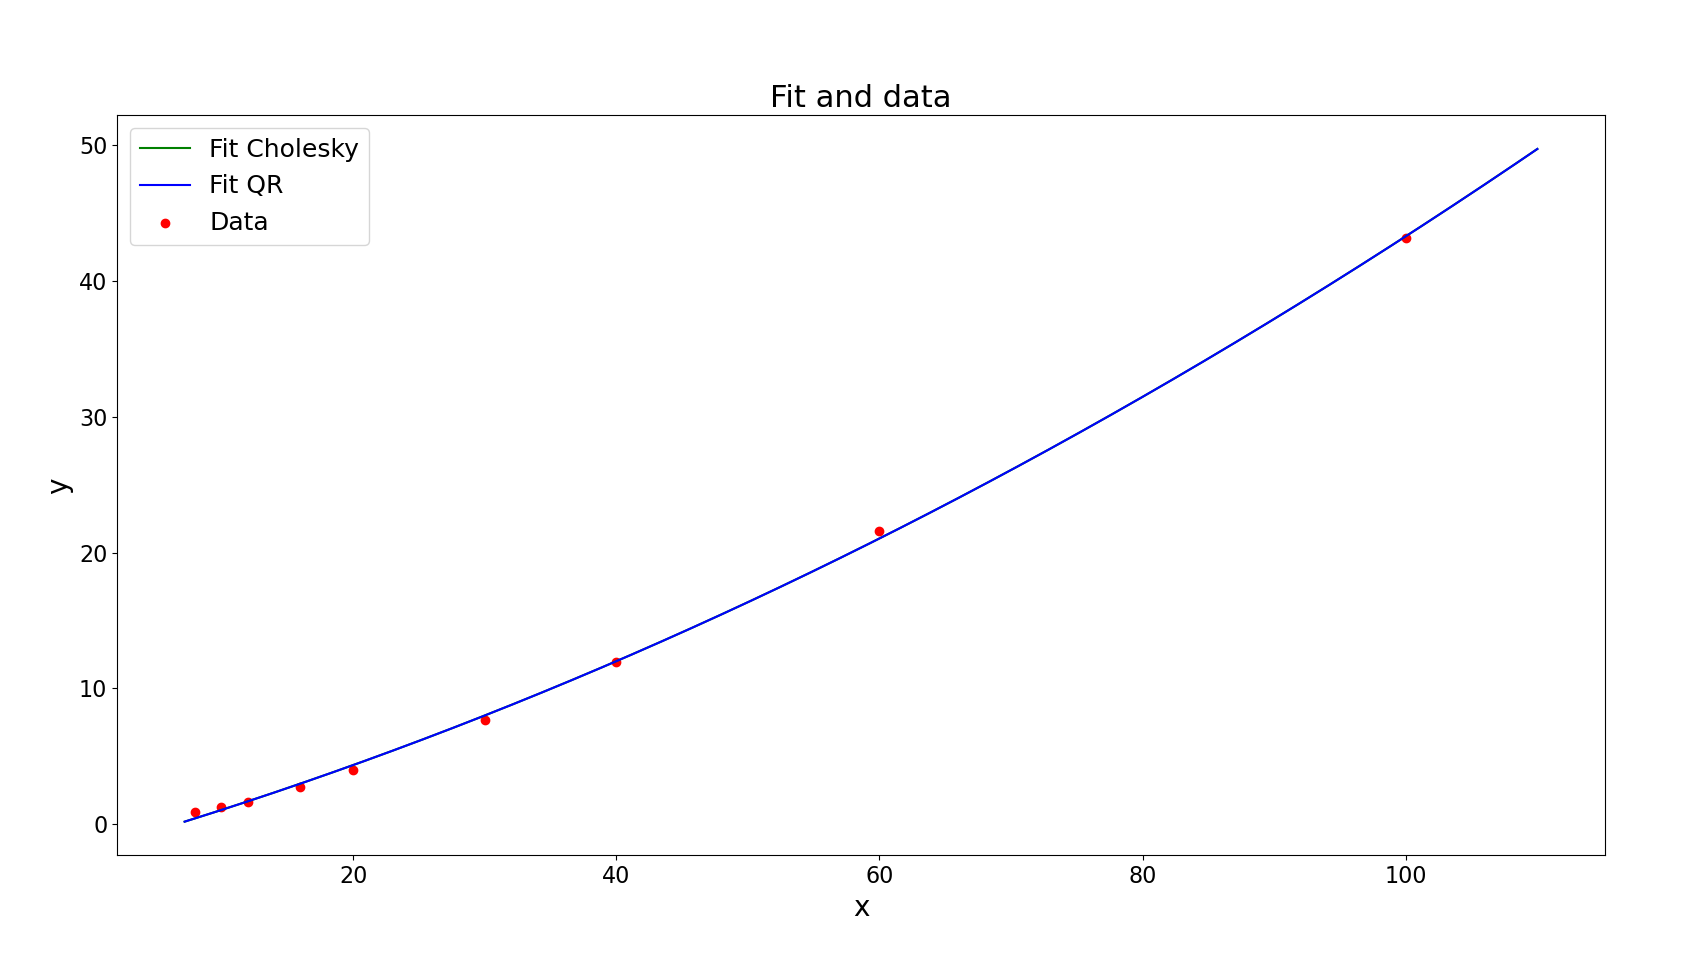
\includegraphics[width=1.1\linewidth]{../Project_2_latex/Plot/Fit_and_data.png}
	\caption{}
	\label{fig: fit and data Cholesky QR}
\end{figure}



\noindent \textbf{(4)} The following code computes the residual $\textbf{r} = \textbf{d} - C\hat{\textbf{x}}$ where $\hat{\textbf{x}} =  \left[  - 1.919,\  0.2782,\  0.001739\right] $ is the approximate solution of the least squares problem.

\noindent ***INSERIRE CODICE***\\

\noindent The results that we obtain are:\\
\begin{tabular}{cc}
 	Residual: &$\textbf{r}  = [ 0.009503999999993,\  0.716895999999906,\ 62.090847999905236]$\\
 	Norm 2 of the residual: &$\lVert  \textbf{r}  \rVert_2 = 62.09498720144942$\\
\end{tabular}.\\
The value of the residual may seem strange, in fact, if we compute the relative error we find:
\begin{equation}\label{key}
	\frac{\lVert  \textbf{x} - \hat{\textbf{x}} \rVert_2 }{\lVert  \textbf{x} \rVert_2 }  = 7.728184292875672\text{e-05}.
\end{equation}

\noindent However, we can observe that, from the relation
\begin{equation}\label{key}
	\frac{1}{k_2(C)} \frac{\lVert  \textbf{r}  \rVert_2 }{\lVert  \textbf{d}  \rVert_2 } \le \frac{\lVert  \textbf{x} - \hat{\textbf{x}} \rVert_2 }{\lVert  \textbf{x} \rVert_2 } \le k_2(C) \frac{\lVert  \textbf{r}  \rVert_2 }{\lVert  \textbf{d}  \rVert_2 }
\end{equation}
we can obtain the following relation for $\textbf{r} $:
\begin{equation}\label{key}
	\frac{\lVert  \textbf{d}  \rVert_2}{k_2(C)} \frac{\lVert  \textbf{x} - \hat{\textbf{x}} \rVert_2 }{\lVert  \textbf{x} \rVert_2 }\le \lVert  \textbf{r}  \rVert_2 \le k_2(C) \lVert  \textbf{d}  \rVert_2 \frac{\lVert  \textbf{x} - \hat{\textbf{x}} \rVert_2 }{\lVert  \textbf{x} \rVert_2 }.
\end{equation}

\noindent With the following python code we have computed the bounds to the residual.
*** INSERIRE CODICE***\\

\noindent From the output of the previous code we know that:
\begin{equation}\label{key}
	5 \times 10^{-7} \lessapprox \lVert  \textbf{r}  \rVert_2 \lessapprox 3 \times 10^9
\end{equation}
this big range is due to the value of $k_2(C)  \simeq 8 \times 10^7$ that suggests us that we should not use the residual to measure the accuracy of the solution when the problem is ill-conditioned as in this case. 

\section*{Problem 2}
\textbf{(1)} Let $A \in \R^{m\times n}$, with $\text{rank}(A) = n$, let {A = QR} be the (full) QR factorization of $A$, with $Q \in \R^{m\times m} $ orthogonal and $R \in \R^{m\times n}$ upper trapezoidal. Also, let $A = Q_1 R_1$ be the reduced QR factorization of $A$ with $Q_1 \in \R^{m\times n}$ having orthonormal columns and $R_1 \in \R^{m\times m}$ upper triangular. Show that $R_1$ is nonsingular, and that the columns $\textbf{q}_1 . . . , \textbf{q}_n$ of $Q_1$ form an orthonormal basis for $\text{Ran}(A)$, the column space of $A$. Also, find an orthonormal basis for $\text{Null}(A^T)$, the null space of $A^T$ .\\
We start showing that $R_1$ is nonsingular. Since $A$ has full rank, we know that:
\begin{equation}\label{key}
	A \textbf{x} = \textbf{0} \Leftrightarrow \textbf{x} = \textbf{0}
\end{equation}
and multiplying both sides for $Q_1^T$ knowing that $Q_1^T Q_1 = \mathcal{I}_n$ we obtain
\begin{equation}\label{key}
	R_1 \textbf{x} = \textbf{0} \Leftrightarrow \textbf{x} = \textbf{0},
\end{equation}
that concludes the proof.\\
Now we want to show that the columns $\textbf{q}_1 . . . , \textbf{q}_n$ of $Q_1$ form an orthonormal basis for $\text{Ran}(A)$. We start observing that 
\begin{equation}\label{key}
	\forall \textbf{y} \in \text{Ran}(A) \exists \textbf{x} \in \R^n : \textbf{y} = A \textbf{x} = Q_1R_1\textbf{x}
\end{equation}
and we know this from the definition of range of a matrix. In a similar way, knowing that $R_1$ is nonsingular and therefore is a bijective map from $\R^n$ to $\R^n$, we can put $\textbf{x}' = R_i \textbf{x}$ and say that:
\begin{equation}\label{key}
	\forall \textbf{y} \in \text{Ran}(A) \exists \textbf{x} \in \R^n : \textbf{y} = A \textbf{x} = Q_1\textbf{x}',
\end{equation}
that means that $\text{Ran}(A) = \text{Ran}(Q_1) = \text{Span}\{\textbf{q}_1,\dots,\textbf{q}_n\}$.\\
Now we want to find an orthonormal basis for $\text{Null}(A^T)$



\section*{Problem 3}

\noindent \textbf{(1)} Let $A \in \R^{m\times n}$, with singular value decomposition $A = U \Sigma V^T = \sum_{i=1}^n \sigma_i \textbf{u}_i \textbf{v}_i^T$ with $\sigma_1 \ge \sigma_2 \ge \dots \ge \sigma_n$ and $\text{rank}(A) = n$. Express the singular values and singular vectors of the following matrices in terms of those of $A$.\\

\textbf{(a)} $(A^{T}A)^{-1}$
\[(A^{T}A)^{-1} = (V^{T})^{-1}\Sigma^{-2}V^{-1}=V\Sigma^{-2}V^{-1}\]
%From this expression we can conclude that:
\begin{itemize}
	\item Both left and right singular vectors of $(A^{T}A)^{-1}$ are equal to the right singular vectors of $A$;
	\item Singular values of $(A^{T}A)^{-1}$ are equal to singular values of $A$ raised to the $-2$ power.
\end{itemize}

\textbf{(b)} $(A^{T}A)^{-1}A^{T}$
\[(A^{T}A)^{-1}A^{T} = V\Sigma^{-2}V^{T}V\Sigma U^{T}=V\Sigma^{-1}U^{-1}\]
\begin{itemize}
	\item Left singular vectors of $(A^{T}A)^{-1}A^{T}$ are equal to the right singular vectors of $A$;
	\item Right singular vectors of $(A^{T}A)^{-1}$ are equal to the left singular vectors of $A$;
	\item Singular values of $(A^{T}A)^{-1}$ are equal to the inverse of singular values of $A$.
\end{itemize}

\textbf{(c)} $A(A^{T}A)^{-1}$
\[A(A^{T}A)^{-1} = U\Sigma V^{T}V\Sigma^{-2}V^{-T}=U\Sigma^{-1}V^{T}\]
\begin{itemize}
	\item Left and right singular vectors of $(A^{T}A)^{-1}$ coincide with that of $A$;
	\item Singular values of $(A^{T}A)^{-1}$ are equal to the inverse of singular values of $A$.
\end{itemize}

\textbf{(d)} $A(A^{T}A)^{-1}A^{T}$
\[A(A^{T}A)^{-1}A^{T} = U\Sigma (V^{T})V\Sigma^{-2}V^{T}V\Sigma U^{T}=\mathbb{1}\]



\noindent \textbf{(2)}

\begin{equation}
	A = \begin{bmatrix}
		1 & 2 \\
		0 & 2
	\end{bmatrix}
\end{equation}

\begin{equation}
	A^{T}A = \begin{bmatrix}
		1 & 2 \\
		2 & 8
	\end{bmatrix}
\end{equation}

\begin{equation}
	\det(A^{T}A -\lambda\mathbb{1})=0
\end{equation}

\begin{equation}
	\lambda_{1,2}=\frac{9 \pm \sqrt{65}}{2}
\end{equation}

\begin{equation}
	k_{2}(A) = \frac{\sigma_{\max}}{\sigma_{\min}} = \sqrt{\frac{9+\sqrt{65}}{9-\sqrt{65}}}
\end{equation}


\end{document}